\chapter{Аналитические выражения}\label{ch:equations}
В данном разделе выполнены аналитические оценки для рассматриваемой задачи пробивания листа обаком осколков.
Оценки проведены по аналогии с пробитием бронежилетов пулями.
Важная особенность состоит в том, что существующие рассчёты проведены в иных скоростных режимах (скорость пули менее
1 $км/c$ ) и при существенно ином пространственном распределении нагрузки (массивный ударник, а не облако мелких
осколков).
Не смотря на это, после некоторой колибровки и сопоставления с экспериментом и численными рассчётами, результаты
аналитических вычислений можно использовать чтобы далее улучшить точность аналитических решений.

В этом разделе рассматривается композитный экран из множества слоёв ткани.
\section*{Параметры}
Параметры волокон ткани приведены в \tabref{tbl:kevlar-params}

\begin{table}[h]
    \centering
    \caption{Параметры ткани}\label{tbl:kevlar-params}
    \begin{tabular}{|l|l|}
        \hline
        Параметр & Значение      \\ \hline
        Плотность & 1430 $кг/м^3$ \\ \hline
        Модуль Юнга & 125 ГПа       \\ \hline
        Предельное удлинение при разрыве & 4.25 \%       \\ \hline
        Прочность на разрыв & 4 ГПа         \\ \hline
        Прочность на сжатие & $40-60$ МПа     \\ \hline
    \end{tabular}
\end{table}

Данные по модулю Юнга, удлинению при разрыве, прочности на разрыв взяты из\cite{perepelkin2009,mikhailin2013}.
Значение прочности на сжатие взято, на основании данных\cite{papkov1986} о том, что прочность параамидных волокон
на сжатие $\approx 1.0 - 1.5 \%$ от прочности на растяжение.

Для пакета принимаем значение пористости: $\mu=0.6$\cite{buzov2004}.

Для облака частиц принимаем характерную скорость $v=4-6$ $км/с$.

\section*{Этапы разрушения пакета}
Исходя из\cite{kobylkin2014} имеем три этапа столкновения ударника с пакетом:

Первый этап -- начало столкновения ударника с пакетом - уплотнение ударника в лицевой части,
ускорение материала в направлении движения ударника.
Разрушение нитей имеет сдвиговый характер.
Смещение слоёв мало.
Торможение ударника незначительно, так как этот этап имеет низкую продолжительность.

Второй этап -- проникновение ударника в пакет.
На этом этапе происходит растяжение и обрыв нитей.
Поперечное смещение велико, деформация превосходит предельную.
На этом этапе происходит торможение ударника и основное поглощение кинетической энергии.

Третий этап -- торможение ударника с образованием купола.
Поглощается оставшаяся часть кинетической энергии.

Для нашего скоростного режима имеет смысл обратить внимание на первые два этапа, так как ожидается полное пробитие пакета.

\subsection*{Волна сжатия}
На начальном этапе столкновения в пакете возникает волна сжатия, в которой происходит поперечное движение слоёв ткани.
В задачах пробивания пакета массивный ударником (пулей) для оценки амплитуды волны сжатия рассматривается приближение,
в котором предполагается, что на фронте фолны происходит уплотнение до сплошного материала.
Воспользовавшись подходом, описаным в\cite{kobylkin2014}, предположим, что плотность изменяется скачком от некоторого
значения $\rho_0$ (с учётом плотности намотки нитей) до значения $\rho_m$ (плотность материала нитей).
\footnote{Следует обратить внимание, что этот приём не до конца обоснован в нашем случае, так как профиль удара сильно
отличается}

Очевидно, что при пористости $\mu$
\begin{equation}
    \rho_0 = (1 - \mu) \cdot \rho_m
\end{equation}
Что для нашего случая даёт: $\rho_m = 570~кг / м^3$

Применяя ЗСМ и ЗСИ для нашего пакета получим:
\begin{equation}
    \rho_0 D = \rho_m (D - u)
\end{equation}
\begin{equation}
    P = \rho_0 u D
\end{equation}
Здесь $D$ -- скорость фронта сжатия, а $u$ -- массовая скорость.

Получим:
\begin{equation}
    D = \frac{u}{\mu}
\end{equation}
\begin{equation}
    P = \frac{\rho_m (1 - \mu) u ^2}{\mu}
\end{equation}

Из этих оценок получаем, что уже при 2 $км/с$ давление будет 4 ГПа, что значительно больше чем прочность на сжатие.
С учётом принятой скорости в $4-6~км/с$ получим, данный процесс будет происходить по всей толщине пакета.

На основании теории\cite{rakhmatulin} и обших подходов и\cite{kobylkin2014} получим оценки для взаимодействия
осколка с нитями тканевого пакета.
При поперечном ударе по нити в ней начинают распространяться продольные и поперечные волны.
При взаимодействии частицы с тканевым пакетом зона высокого давления ограничена радиусом отрыва поперечной волны
в нитях ткани от поверхности частицы.
До отрыва поперечной волны от частицы общая конфигурация взаимодействия соответствует изображённой на
\picref{fig:first-stage}, а после - изображённой на \picref{fig:second-stage}

\begin{figure}[H]
    \centering

    \caption{Конфигурация до отрыва поперечной волны}
    \label{fig:first-stage}
    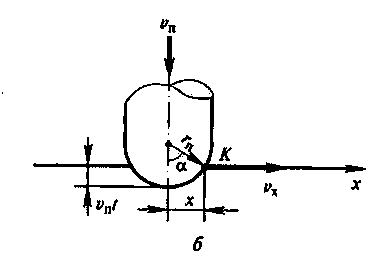
\includegraphics[width=0.5\textwidth]{img/first_stage.png}

    \caption{Конфигурация после отрыва поперечной волны}
    \label{fig:second-stage}
    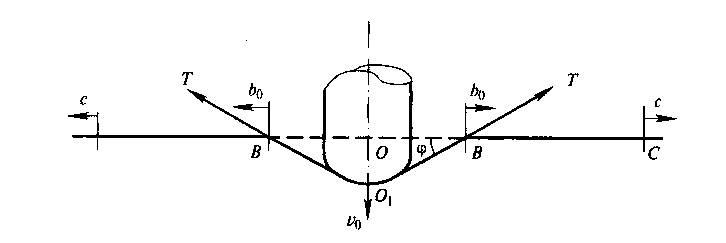
\includegraphics[width=0.8\textwidth]{img/second_stage.png}
\end{figure}

Для сферической